\section{Rechnungsbsp}
\subsection{B2U RL}
\begin{minipage}{0.4\linewidth}
    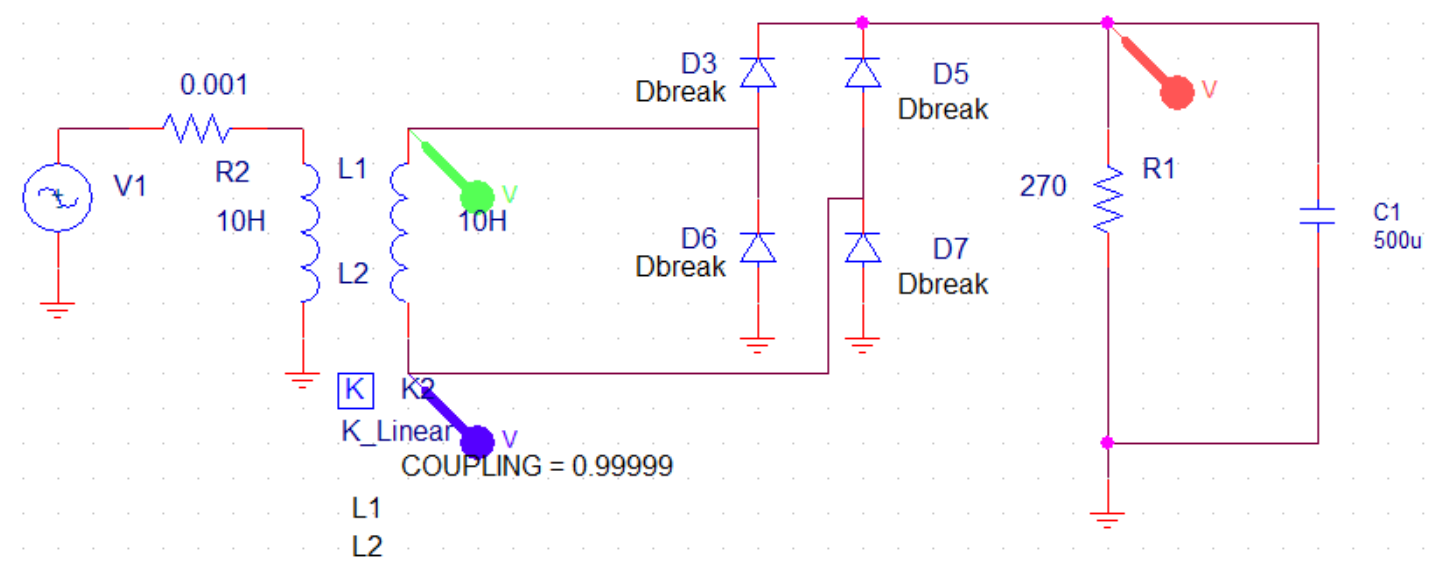
\includegraphics[width=\linewidth]{images/Rechnungsbsp/B2URC}
\end{minipage}
\begin{minipage}{0.2\linewidth}
    \includegraphics[width=\linewidth]{images/Rechnungsbsp/B2URCKl}
\end{minipage}
\begin{minipage}{5cm}
   $ R = 270 $ \newline
   $ C = 500 \cdot 10^{-6} $\newline
   $ U_{2m} = 30 $ \newline
   $ f = 50 Hz $   
\end{minipage}
\newline
\textbf{Diode Sperrt:} $ U_R > U_2 \quad \rightarrow \quad $ Sperrwinkel $\alpha$ $\qquad \alpha \leq \beta \leq \gamma$
\begin{align*}
     0 & = i_R + i_C \\
     0 & = \frac{U_R}{R}+ C \frac{\diff U_R}{\diff t} \qquad \tau = RC \qquad t = \frac{\beta}{\omega}\\
     - \frac{t}{\tau} + A & = \frac{1}{U_R} \diff U_R \\
     U_R(\beta) & = B \cdot e^{-\frac{\beta}{\omega \tau}}
     \end{align*}
 Um B herauszufinden müssen die Anfangsbedingungen eingesetzt werden.\newline 
 Beim Winkel $\alpha$ ist der Spg-Verlauf von $U_2$ = der StartSpg. 
     \begin{align*}
     U_R(\alpha) & =U_R(\alpha)\\
     U_{2m} \cdot sin(\alpha) & = B \cdot e^{-\frac{\alpha}{\omega \tau}}\\
     B & = U_{2m} \cdot sin(\alpha) \cdot e^{\frac{\alpha}{\omega \tau}}\\
     U_R(\beta) & =  U_{2m} \cdot sin(\alpha) \cdot e^{-\frac{\beta - \alpha}{\omega \tau}} \qquad \alpha \leq \beta \leq \gamma       
\end{align*}
Als nächstes müssen wir $\alpha$ bestimmen. Sobald die Steigung von $U_R \neq U_{2}$ sperrt die Diode $\alpha = \beta$
\begin{align*}
    U_R(\beta) \frac{\diff}{\diff \beta} & = U_2(\beta) \frac{\diff}{\diff \beta}\\
    \left( U_{2m} \cdot sin(\alpha) \cdot e^{-\frac{\beta - \alpha}{\omega \tau}}\right)\frac{\diff}{\diff \beta} & = \left( U_{2m} \cdot sin(\beta)\right)\frac{\diff}{\diff \beta}\\
    U_{2m}\cdot sin(\alpha)\cdot e^{\frac{\alpha - \beta}{\omega \tau}}\cdot \frac{-1}{\omega \tau} &= U_{2m}\cdot cos(\beta) \qquad | \alpha = \beta\\
    sin(\alpha)\cdot \frac{-1}{\omega \tau} &= cos(\alpha)\\
    \alpha & = -arctan(\omega \tau) \qquad 0 < \alpha < \pi\\
    \alpha & = -1.547 \qquad \pi -Periodisch\\
    \alpha & = 1.5943 \rightarrow 91.35_{grad}
\end{align*}

\textbf{Diode leitet:} $ U_R < U_2 \quad \rightarrow \quad $ Durchlasswinkel $\gamma \qquad \gamma \leq \beta \leq \alpha$
\begin{align*}
    U_2(\gamma) & = U_R(\gamma)\\
    U_{2m}\cdot -sin(\gamma) & = U_{2m} \cdot sin(\alpha) \cdot e^{-\frac{\gamma - \alpha}{\omega \tau}}\\
    -sin(\gamma) & = sin(\alpha) \cdot e^{\frac{\alpha - \gamma}{\omega \tau}} \qquad \pi < \gamma < \nicefrac{3\pi}{2}\\
    \gamma & = 4.354 \rightarrow 249.5_{grad}
\end{align*}

\textbf{Diode leitet} $ \gamma - \pi = 69_{grad} < \beta < \alpha = 91.35_{grad} $\newline
\[  U_R(\beta) = U_{2m} \cdot sin(\beta)\]

\textbf{Diode sperrt} $ \alpha = 91.35_{grad}< \beta < \gamma = 249.5_{grad}  $\newline
\[  U_R(\beta)  =  U_{2m} \cdot sin(\alpha) \cdot e^{-\frac{\beta - \alpha}{\omega \tau}}\]
